\documentclass[letterpaper, 10 pt, conference]{article} 
\usepackage[english]{babel}
\usepackage{amsmath,amssymb,amscd,amsthm} % variety of useful math macros
\usepackage[inner=1.5 cm, outer = 1.5 cm, top=1 cm, bottom = 1.5 cm]{geometry}
\usepackage{subcaption}
%For inserting graphics
\usepackage{graphicx}
\usepackage[dvipsnames]{xcolor}
\usepackage{listings}
\usepackage[utf8]{inputenc}
\usepackage{hyperref}
\usepackage{array, multirow}
\usepackage{lipsum}
\usepackage{natbib}
\usepackage[normalem]{ulem}


\bibliographystyle{abbrvnat}

\newtheorem{thm}{Theorem}
\newtheorem{prop}{Proposition}
\newtheorem{lemma}{Lemma}
\newtheorem{ex}{Exercise}
\newtheorem{exm}{Example}
\newtheorem{defn}{Definition}

\newcommand\E{\ensuremath{\mathbb{E}}}
\newcommand\N{\ensuremath{\mathbb{N}}}
\renewcommand{\P}{\ensuremath{\mathbb{P}}}
\newcommand\Q{\ensuremath{\mathbb{Q}}}
\newcommand\R{\ensuremath{\mathbb{R}}}
\newcommand\Z{\ensuremath{\mathbb{Z}}}

\newcommand\var[1]{\, \mathrm{Var} \left( #1 \right)}

\newcommand\pr[1]{\, \mathbb{P} \left\lbrace #1 \right\rbrace}

\newcommand\cov[1]{\, \mathrm{Cov} \left( #1 \right)}

\newcommand\expec[1]{\, \mathbb{E} \left\lbrack #1 \right\rbrack}

\title{Central Limit Theorem
}
\date{December 8, 2020}

\hypersetup{
	colorlinks=true,
	linkcolor=blue,
	filecolor=magenta,      
	urlcolor=blue,
	citecolor=MidnightBlue
}

\author{Gerardo {\textsc{Palafox}}}

\begin{document}
\maketitle
\begin{abstract}
	In this work, the central limit theorem is presented, along some applications of the same.
\end{abstract}
\section{Introduction}
First, a definition concerning convergence of random variables is given. With this, the central limit theorem (CLT) can be stated. The proof is omitted but can be seen in the work of \cite{Casella_Berger_2002}. In Section \ref{section:markov}, an application of the  CLT to Markov chains is explained. Then, an application of the central limit theorem to defining and detecting hierarchical community structures in networks is given in Section \ref{section:community}. Finally, in Section \ref{section:epidemics}, a CLT for an SIR epidemics in a configuration model is discussed.

\subsection{Basic theory}

\begin{defn}
	A sequence of random variables $X_1, X_2, \dots,$ converges in distribution to a random variable $X$ if 
	\begin{equation}
		\lim_{n \rightarrow \infty} F_{X_n} (x) = F_X (x)
	\end{equation}
	at all points $x$ where $F_{X} (x)$ is continuous.
\end{defn} 

\begin{thm}[Central limit theorem \citep{Casella_Berger_2002}]
Let $X_1, X_2, \dots$ be a sequence of i.i.d. random variables with $\expec{X_i}  = \mu$ and $0 < \var{X_i} = \sigma^2 < \infty$. Define $\bar{X}_n = (1/n) \sum_{i = 1}^{n} X_i$. Let $G_n (x)$ denote the cumulative distribution function of $\sqrt{n} (\bar{X}_n - \mu)/\sigma$. Then, for any $x$,
\begin{equation}
	\lim_{n \rightarrow \infty} G_n (x) = \int_{-\infty}^{x} \frac{1}{\sqrt{2 \pi}} e^{-y^2 / 2} \, dy ;
\end{equation}
that is, $\sqrt{n} (\bar{X}_n - \mu)/\sigma$ converges in distribution to a standard normal random variable.
\end{thm}

\section{Markov Chains}\label{section:markov}
A stochastic process is a sequence of random variables $\lbrace X_i \rbrace_{i \in I}$. A Markov chain is a stochastic process that takes on a finite or countable number of possible values, called states, and such that 
\begin{equation}
	\pr{X_{n+1} = j | X_{n} = i, X_{n-1} = i_{n-1} , \dots, X_1 = i_1, X_0 = i_0} = \pr{X_{n+1} = j | X_{n} = i}.
\end{equation}
Markov chains have several applications, for example, modeling of epidemic processes, such as the one described in Section \ref{section:epidemics}. More about the basic theory of Markov chains can be found in the texts of \citet{Ross_2000, feller, lawler_2006}. For a state $i$, let $f_i$ denote the probability that, starting at state $i$, the process will ever reenter state $i$. If $f_i = 1$, state $i$ is said to be \textit{recurrent}, and if $f_i < 1$, the state is said to be \textit{transient} . If state $i$ is recurrent, starting in state $i$, the process will enter state $i$ infinitely often.
Let $k$ be a recurrent state in a finite Markov chain. Let $N_n$ denote the number of passages up to time $n$ of the system through state $k$. Then, $N_n$ is normally distributed as $n \rightarrow \infty$ \citep{feller}. For example, consider a Markov chain with states $\lbrace 0, 1 \rbrace$ and probabilities $\pr{X_{n+1} = j | X_{n} = i} = P_{ij}$ given by the entries of the matrix
\begin{equation}
P = 
	\begin{bmatrix}
	.3 & .7 \\
	.6 & .4
	\end{bmatrix}.
\end{equation}
Then the number $N_{n}$ of passages up to time $n$ of the system through the state 0 is normally distributed as $n \rightarrow \infty$. This Markov chain was simulated\footnote{The code of this simulation, as well as this report, can be found in the Github repository \url{https://github.com/palafox794/AppliedProbabilityModels/tree/master/Assignment14}} in R \citep{R} on a Jupyter notebook \citep{jupyter}. The number $N_n$ for $n = 10,000$ was computed a thousand times. The histogram of these results is shown in Figure \ref{fig:hist}.

\begin{figure}
\centering
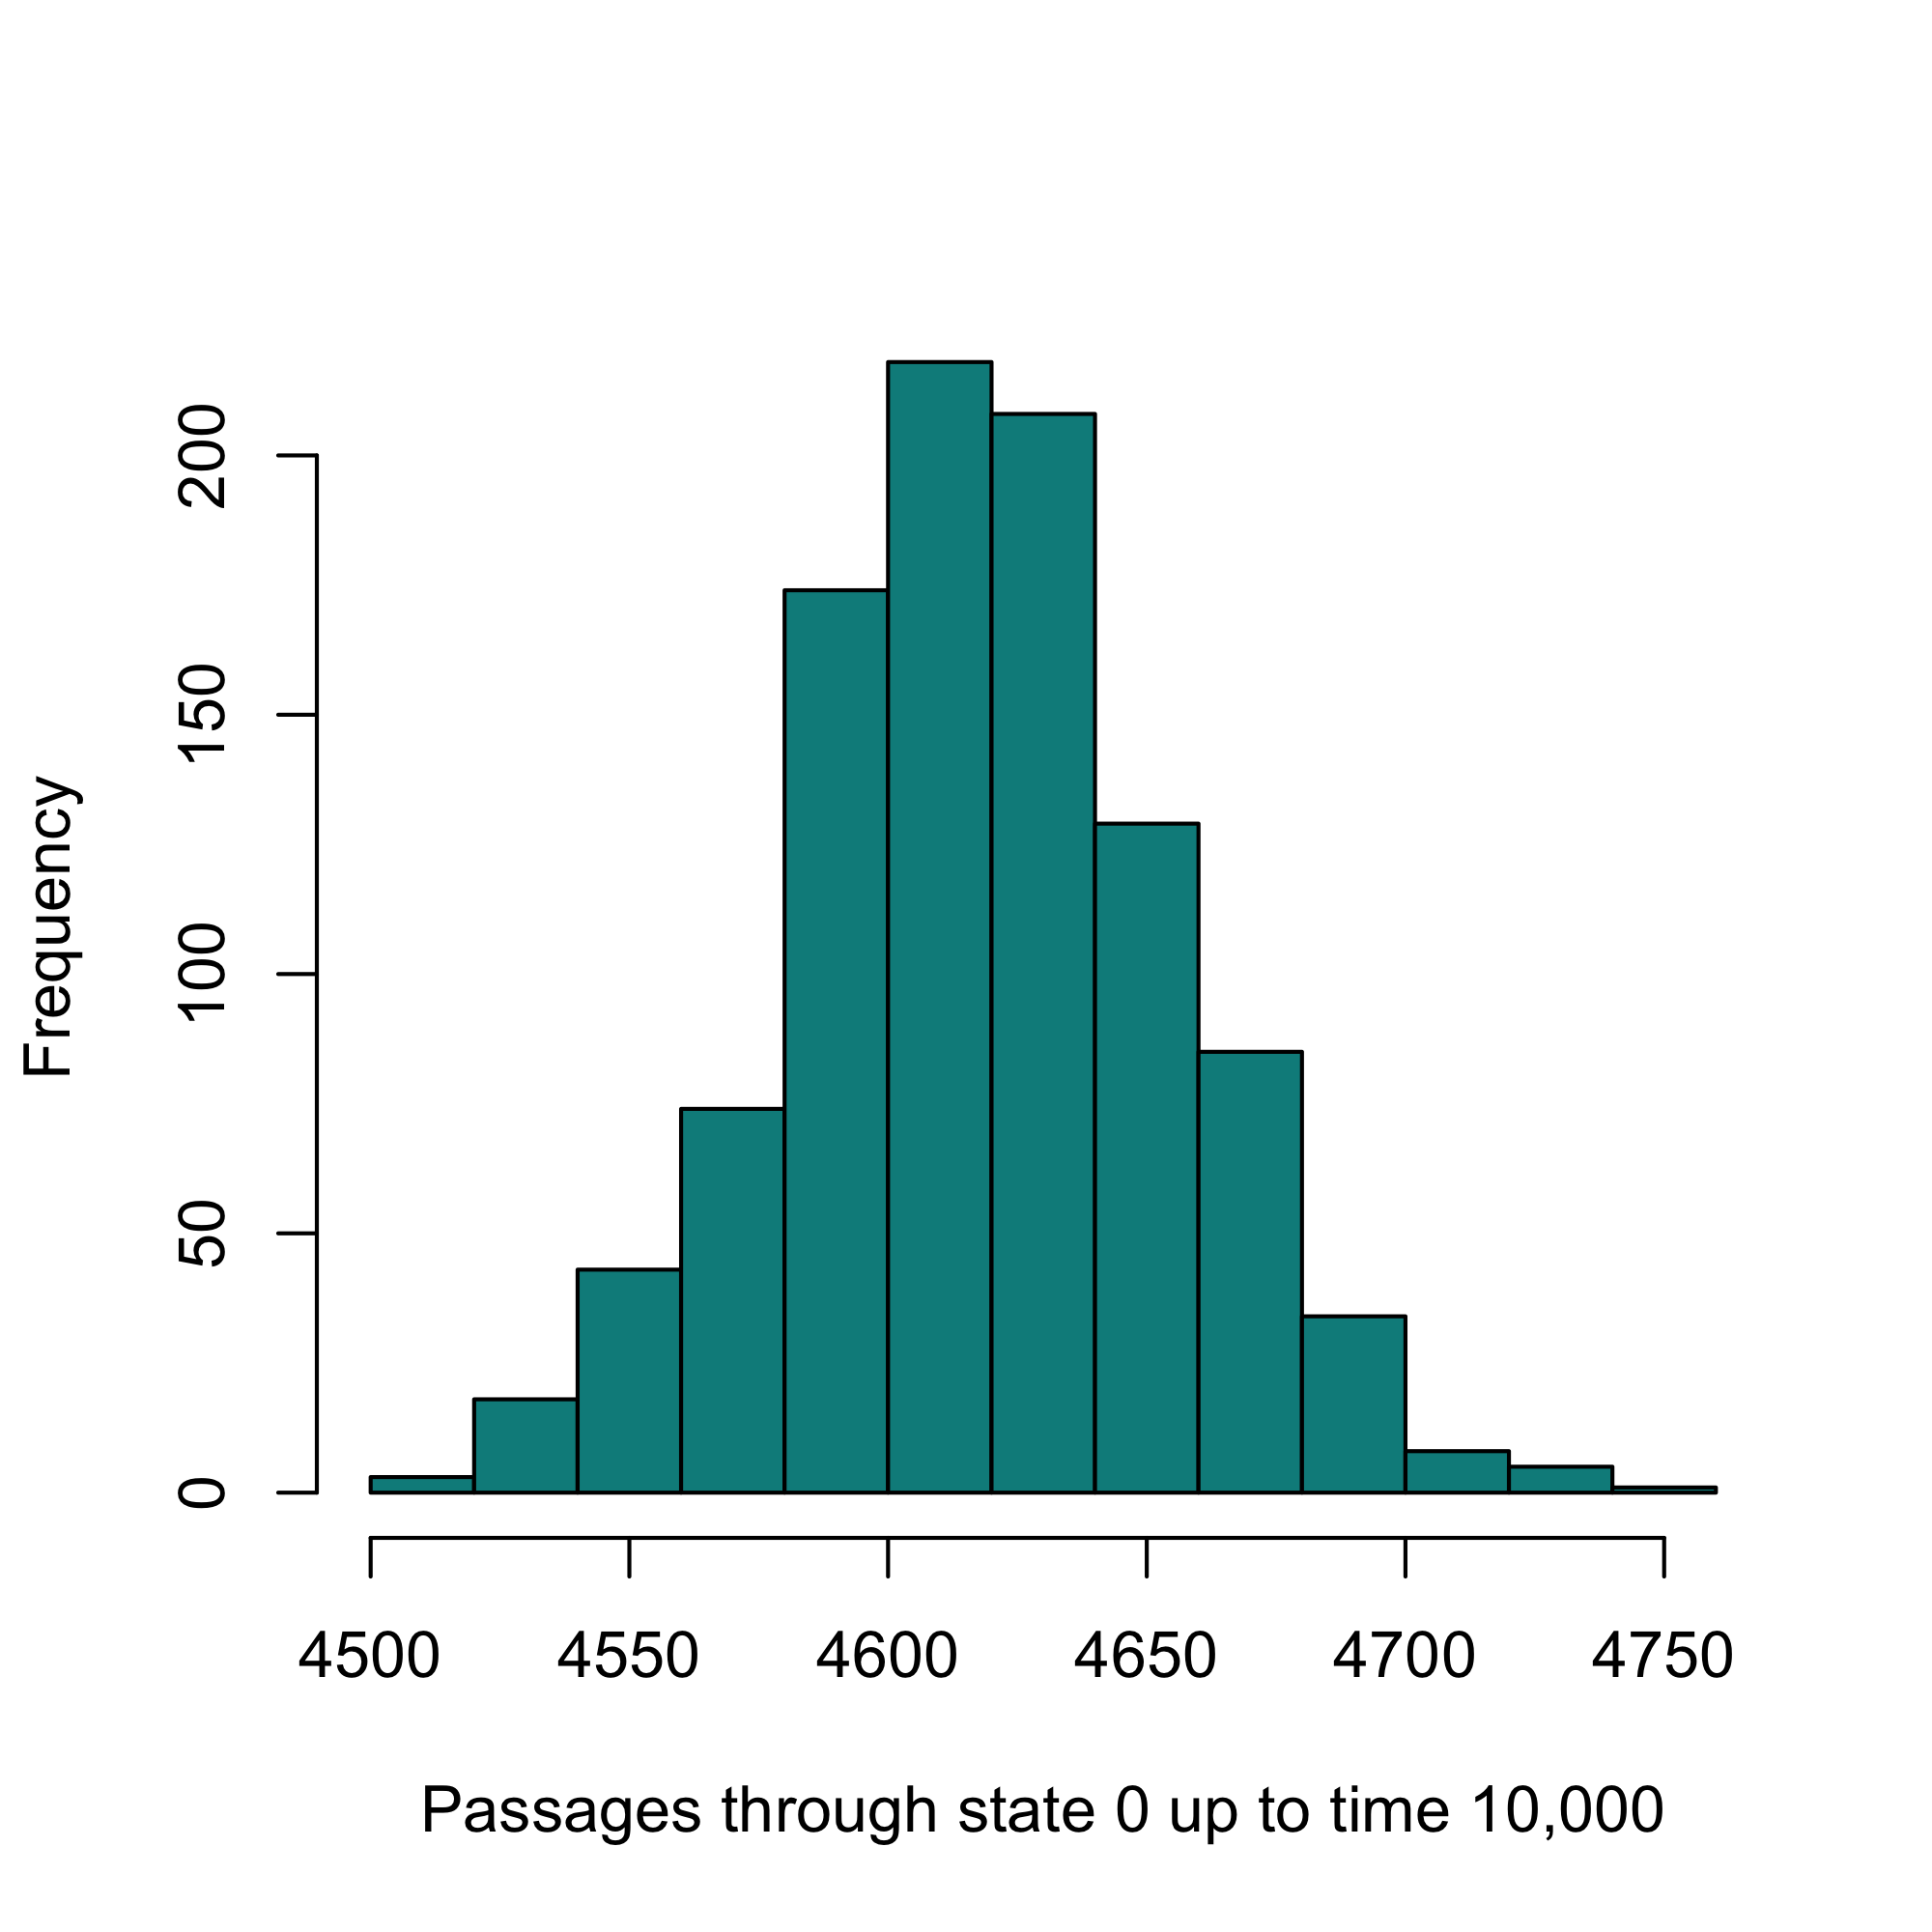
\includegraphics[width =.5\linewidth]{hist}
\caption{Histogram of $N_n$ for large $n$.}
\label{fig:hist}
\end{figure}

\section{Hierarchical community structure in networks}\label{section:community}
\citet{schaub2020hierarchical} studied hierarchical community structures in networks. In particular, their work addresses how to define hierarchies of communities, how to determine if such hierarchical structure exists in a network, and how to detect such structures efficiently. To define similarities between nodes, some terminology is introduced. Groups of nodes $r$ and $s$ are called \textit{stochastically equivalent} if any node in group $r$ has the same probability $\Omega_{rs}$ of linking to any node in group $s$. Then, the stochastic block model (SBM) is used to represent the community structure of a network. The SBM defines the probability of a link existing between two nodes depending on their community assignment, with a group indicator binary matrix $H$, where $H_{ir} = 1$ if node $i$ is assigned to group $r$ and $H_{ir} = 0$ otherwise. Denoting by $H_{i \cdot}$ the $i$th row of $H$, $A$ the adjacency matrix of the network, and $\Omega$ the affinity matrix,  the probability of nodes $i$ and $j$ being linked is given by 
\begin{equation}
\pr{A_{ij} = 1} = H_{i \cdot} \Omega H_{j \cdot}^{\top}.
\end{equation}
The SBM provides a parametric probability distribution over adjacency matrices. The expected adjacency matrix of this distribution can be calculated from the affinity matrix $\Omega$ and group indicator matrix $H$ as 
\begin{equation}
	\expec{A} = H \Omega H^\top.
\end{equation}
Nodes in the network $\expec{A}$ which are in the same group are caled \textit{structurally equivalent}.  A partition of an adjacency matrix $A$ such that every node in a group $r$ has the same number of links to nodes in a group $s$ is called an \textit{equitable partition}.  A \textit{stochastic equitable partition} is an equitable partition in expectation. Partitions that are equitable only between different groups are called \textit{externally equitable partitions} (EEP). A \textit{stochasitc externally equitable partition} (sEEP) is a partition that is externally equitable in expectation.  A hierarchical partition is a \textit{valid hierarchy} if at each level the partition is a sEEP and is not degenerate.  
In detecting hierarchies via spectral methods, authors approximate the true affinity matrix via an estimated affinity matrix $\hat{\Omega}$.
To measure how well a partition of $\hat{\Omega}$ approximates an EEP of $\Omega$, the authors use the central limit theorem to conclude the spectral properties of $\hat{\Omega}$ will closely approximate the true $\Omega$, since for large $n$ the entry $\hat{\Omega}_{ij}$ will be approximated by a normal $\mathrm{N}(\mu_{ij}, \sigma_{ij})$ random variable, and $\mu_{ij} = \Omega_{ij}$, $\sigma^{2}_{ij} = \Omega_{ij} (1-\Omega_{ij}) / n_i n_j$, where $n_i, n_j$ are the number of nodes in group $i$ and $j$ respectively.  

%%%%%%%%%%%%%%%%%%%%%%%%%%%%%%%%%%%%%%%%%%%%%%%%%%%%%%%%%%%%%%%%%%%%%%%%%%%%%%%%
\section{Central limit theorems for SIR epidemics on random graphs}\label{section:epidemics}
\citet{ball2018central} develops central limit theorems for a stochastic susceptible - infectious - recovered epidemic defined on a configuration model \citep{Newman_2018} random graph. Graphs where degrees of individuals are deterministic (Molloy-Reed) and where degrees are i.i.d. (Newman-Strogatz-Watts) are considered. A population of $n$ individuals, labeled $1, 2, \dots, n$, is considered. Let $T_{i}^{(n)}$ be the total number of degree-$i$ susceptibles infected by the epidemic, and $T^{(n)} = \sum_{i = 0}^{d_\text{max}} T_{i}^{(n)}$ the final size of the epidemic, where $d_\text{max}$ is the maximum degree among all nodes. Upon a suitable standardization, it is proven that the final size of the epidemic converges in distribution to a normal random variable.  Let $a_{i}^{(n)}$ be the number of degree $i$ initial infectious, and $a^{(n)} = \sum_i a_{i}^{(n)}$ the total number of initial infectious. Let  $\epsilon^{(n)} = n^{-1} a^{(n)}, \epsilon_{i}^{(n)} = n^{-1} a_{i}^{(n)}, \epsilon := \lim_{n \rightarrow \infty} \epsilon^{(n)}$, and let $\epsilon_i$ be such that $\lim_{n \rightarrow \infty} \sqrt{n} (\epsilon_{i}^{(n)} - \epsilon_i)  =0$. If the degree distribution is a random variable $D$, let $\pr{D = i} = p_i$ and $\mu_D = \expec{D}$. Let $p_I$ be the probability that the neighbor of an infectious individual is contacted, and $q_I = 1 - p_I$ the probability that an infectious fails to contact a given neighbor. Let $f_{D_{\epsilon}} (s) = \sum_{i = 0}^{d_\text{max}} (p_i - \epsilon_{i})s^i$. Define $z \in [0,1)$ as the unique solution of 
\begin{equation}
	z - q_I = \mu_{D}^{-1} p_I f_{D_\epsilon} (z),
\end{equation}
and 
\begin{equation}
	\rho = 1 - \epsilon - f_{D_\epsilon} (z).
\end{equation}
It is proven \citep{ball2018central} that $\sqrt{n} (n^{-1} T^{(n)} - \rho)$ converges in distribution to a normal random variable.



%%%%%%%%%%%%%%%%%%%%%%%%%%%%%%%%%%%%%%%%%%%%%%%%%%%%%%%%%%%%%%%%%%%%%%%%%%%%%%%%
\bibliography{ref}

\end{document}
